\documentclass[a4paper,english, oneside, 12pt]{memoir} %kan laves til twoside
\chapterstyle{southall}
\usepackage[T1]{fontenc}
\usepackage[applemac]{inputenc}
\usepackage[english]{babel}
\usepackage{amsmath,amssymb,amsthm}
\numberwithin{equation}{section} 
\usepackage{booktabs,dcolumn,cellspace}
\usepackage{graphicx} %[pdftex]
\usepackage{wrapfig}
\usepackage{placeins} %float barrier
\usepackage[margin=3cm]{geometry} 
\setsecnumdepth{subsubsection}
\setcounter{tocdepth}{2}
\linespread{1.0}
\usepackage{array,booktabs}
\usepackage{caption}
\usepackage{subfig}
\usepackage{lscape}
\usepackage{array}
\usepackage{pbox}
\usepackage{lastpage}
%\usepackage{rotfloat}
\usepackage{multirow}
\usepackage{color}
\usepackage{relsize} 
\usepackage{fancyvrb}
\usepackage{tabularx}
\usepackage{rotating}
\usepackage{framed}
\usepackage{longtable}
\setlength{\parindent}{0pt}
\nonzeroparskip
\usepackage{lipsum}
\usepackage{listings}
\usepackage{algpseudocode}
\usepackage{textcomp}
\usepackage{hyperref}
\hypersetup{linktocpage}
\hypersetup{colorlinks,citecolor=red,filecolor=blue,linkcolor=red,urlcolor=blue}
\captionsetup[subfigure]{margin=10pt, parskip=0pt,hangindent=0pt, indention=0pt, singlelinecheck=true} 
\captionsetup[figure]{format=hang,justification=raggedright} %ndrer p caption pakken
\captionsetup{format=hang,justification=raggedright} %ndrer p caption pakken
\captionsetup[figure]{font={footnotesize,sf},labelfont=bf, singlelinecheck=1, width=0.85\textwidth}
\captionsetup[figure]{labelfont={bf,small},textfont={small}}
\captionsetup[subfloat]{labelfont={bf,small},textfont={small},
subrefformat=parens}
\usepackage{lineno}
\usepackage{minted}
\providecommand{\inlinecode}[1]{\texttt{#1}}
\providecommand{\todo}[1]{\addcontentsline{tdo}{todo}{\protect{#1}}\marginpar{\textcolor{red}{#1}}}
\newcommand{\tab}[1]{\hspace{.2\textwidth}\rlap{#1}}
\newcommand{\myparagraph}[1]{\paragraph{#1}\mbox{}\\}
\definecolor{listinggray}{gray}{0.9}
\definecolor{lbcolor}{rgb}{0.9,0.9,0.9}
\lstset{
	backgroundcolor=\color{lbcolor},
	tabsize=4,
	rulecolor=,
	language=matlab,
        basicstyle=\scriptsize,
        upquote=true,
        aboveskip={1.5\baselineskip},
        columns=fixed,
        showstringspaces=false,
        extendedchars=true,
        breaklines=true,
        prebreak = \raisebox{0ex}[0ex][0ex]{\ensuremath{\hookleftarrow}},
        frame=single,
        showtabs=false,
        showspaces=false,
        showstringspaces=false,
        identifierstyle=\ttfamily,
        keywordstyle=\color[rgb]{0,0,1},
        commentstyle=\color[rgb]{0.133,0.545,0.133},
        stringstyle=\color[rgb]{0.627,0.126,0.941},
}

\makepagestyle{plain}
\makeevenfoot{plain}{}{\thepage\ of \pageref*{LastPage}}{}
\makeoddfoot{plain}{}{\thepage\ of \pageref*{LastPage}}{}


\renewcommand\chapterheadstart{\vspace*{1 pt}}
\pagestyle{plain}


\begin{document}

\frontmatter
\begin{titlingpage}

\centering \parindent=0pt
\newcommand{\HRule}{\rule{\textwidth}{1mm}}
\vspace*{\stretch{1}} \HRule\\[1cm]
\Huge\bfseries TAPY\\[0.7cm]
\large Type Analysis for Python \\[1cm]
\HRule\\[2cm] \large Jesper Lindstr\o m Nielsen - \texttt{jesper.jln@gmail.com} \\
\large Christoffer Quist Adamsen - \texttt{christofferqa@gmail.com} \\
\large Troels Leth Jensen - \texttt{troelslethjensen@gmail.com} \\

\vspace*{2 cm}  \normalsize 

\begin{flushleft}
Aarhus University\\
May 3, 2013 \end{flushleft}




\end{titlingpage}

%\tableofcontents

\mainmatter
\chapter*{Abstract}
We present a proof of concept for doing type analysis for Python using the monotone framework. We present how some interesting language features are converted into control flow graphs (CFGs), and also how it is possible to dynamically extend a CFG with calls to the so-called magic methods during the analysis, in order to minimize the total CFG in which the analysis works on. Finally, we show that our type analyser is able to analyse small programs that involves non-trivial language features that distinguishes Python from other dynamic languages, e.g. JavaScript.
\chapter{Introduction}
Python is a dynamically typed, general purpose programming language that supports both object-oriented, imperative and functional programming styles.

Python has a lot of similarities to JavaScript as they are both dynamic languages. However, static type analysis of Python is further complicated by its scoping rules \cite{lambdapy}, magic methods, generator expressions and others. One of the reasons why magic methods are challenging to reason about, is that they result in implicit method and function calls; this makes it harder to predict the outcome of, otherwise relatively, simple statements and expressions, e.g. attribute lookup.

Python is widely used in both education and industry, and because of this popularity IDEs \cite{ide.appcelerator, ide.jetbrains, ide.wingware} and other third-party tools \cite{tool.pep8, tool.pyflakes, tool.pychecker, tool.pylint} have been developed to accommodate the developer by finding errors and making refactorings. Sadly, all these tools are affected by the complexity in the Python language and shown to be unsound \cite{lamdapy}. In this report we present our work towards developing a conservative and sound type analysis for Python version 2.7.5\footnote{This version is still predominantly used in the wild.} written in Scala, furthermore we use the third-party project Jython \cite{jython} to parse Python.

\section{Aims and Contributions}
Inspired by Type Analysis for JavaScript (TAJS) \cite{tajs} our aim for this project is to develop a type analysis for Python that will be able to analyze simple Python programs for type related errors. Especially, we wish to be able to do type analysis on programs that use the magic method \inlinecode{\_\_getattr\_\_}, which is called whenever an attribute lookup results in an \inlinecode{AttributeError}. In order to achieve this goal our type analyzer should be able to handle declarations and instantiations of classes, exceptions and others.

This report presents a proof of concept that static analysis of Python is possible using the traditional monotone framework. We present how to construct CFG snippets for various statements and expressions, including a dynamic way to change the CFG during execution of the analysis to accommodate the support for the magic method \inlinecode{\_\_getattr\_\_}.  

During the development of our project we have identified some intriguing features in Python, that includes its scope rules and the order of evaluation when handling magic methods.

\section{Dynamic features and type related errors}
\label{Features}
In this section we give some examples of typical type errors that may occur in Python programs.

Classes can be modified after creation. The code in \autoref{code:Features1} declares a class \inlinecode{Student} with a constructor that inherits from the builtin class \inlinecode{object}.

\begin{listing}[H]
  \begin{minted}[linenos]{python}
class Student(object):
  def __init__(self, name):
    self.name = name
s1 = Student('Foo')
s2 = Student('Bar')
def addGrade(self, course, grade):
  self.grades[course] = grade
Student.addGrade = addGrade
s1.grades = {}
s1.addGrade('math', 10)
s2.addGrade('math', 7)
  \end{minted}
  \caption{Magic method example in Python}
  \label{code:Features1}
\end{listing}

At line 8 a function \inlinecode{addGrade} is written to the \inlinecode{addGrade} attribute of the \inlinecode{Student} class. Since it is written onto a class it will be wrapped in an unbound method; this will ensure that the function can be called as a method on instance objects; especially, the receiver object will be implicitly passed to the \inlinecode{self}\footnote{The first argument is not required to be called \inlinecode{self}, but it is considered bad practice to name it otherwise.} argument (eliminating the purpose of having the \inlinecode{this} keyword as in e.g. JavaScript).

At line 9 the attribute \inlinecode{grades} is set to an empty dictionary on the \inlinecode{s1} object. Therefore we can call the (bound) method \inlinecode{addGrade} on the \inlinecode{s1} object without getting a runtime error. However, since we forgot to set the \inlinecode{grades} attribute on the \inlinecode{s2} object, we will get the following runtime error from line 11: \inlinecode{AttributeError:\ 'Student' object has no attribute 'grades'}. 

Recall that the receiver object is given implicitly as a first argument to the \inlinecode{addGrade} method. 
In case we had forgotten to supply the extra formal parameter \inlinecode{self}, the following runtime error would result from line 10:
\inlinecode{TypeError:\ addGrade() takes exactly 2 arguments (3 given)}. 

% Another interesting aspect with regards to parameter passing is that Python supports unpacking of argument lists. For instance we could have provided the arguments to the \inlinecode{addGrade} function in line 10 by means of a dictionary instead: \inlinecode{s1.addGrade(**\{ 'course': 'math', grade: 10\})}.

However, a type error would occur if line 9 was changed to \inlinecode{s1['grades'] = \{\}} (as is possible in JavaScript), namely: 
\inlinecode{TypeError:\ 'Student' object does not support item assignment}. Additionally, trying to access \inlinecode{s1['grades']} would result in the following error: \inlinecode{TypeError:\ 'Student' object has no attribute '\_\_getitem\_\_'}. Instead this could be achieved by calling the built-in functions \inlinecode{getattr(obj, attr)} and \inlinecode{setattr(obj, attr, val)}.

Python does however allow the programmer to customize the behavior when indexing into an object by supplying the magic methods
\inlinecode{\_\_setitem\_\_} and \inlinecode{\_\_getitem\_\_}, giving the programmer much more freedom. As an example consider the new Student class below:

\begin{listing}[H]
\begin{minted}[linenos]{python}
class Student(Person):
  def __getitem__(self, name):
    return self.grades[name]
  def __setitem__(self, name, val):
    setattr(self, name, val)
  def __getattr__(self, name):
    if name in self.grades:
      return self.grades[name]
    else:
      return "<no such grade>"
\end{minted}
	\caption{Magic method example in python}
	\label{code:Features2}
\end{listing}

With this implementation we could set the \inlinecode{grades} attribute as in JavaScript: \inlinecode{s1['grades'] = \{\}} (due to the implementation of \inlinecode{\_\_setitem\_\_}), and get the grade of \inlinecode{s1} in the math course by calling \inlinecode{s1.math} (due to \inlinecode{\_\_getattr\_\_}) or \inlinecode{s1['math']} (due to \inlinecode{\_\_getitem\_\_}). This is exactly one of the reasons why Python is so difficult to statically analyze: even something as fundamental as attribute lookups possibly involves several method invocations.

As mentioned we want our type analyzer to support the magic method \inlinecode{\_\_getattr\_\_} which comes into play when accessing attributes on class instances, as we illustrated above. In the section about magic methods we describe in detail what exactly happens, together with our work towards supporting this particular magic method.
\chapter{Limitations}

Rather than going with the latest version of Python, we will be working on version 2.7. This version is still predominantly used in the wild and we were only able to find a ready-to-use parser for 2.7 which, given the scope of this project, was a huge selling point. The magic methods remain unchanged in the 3.x family, so extending this proof of concept for a more recent version is straightforward.

\section{Language features}
Python is a general purpose programming language and quite popular, it has been developed and extended and holds a lot of different functionality, some of these functionalities is not used that often. In our analysis we have decided to exclude some of these language functionalities;

\begin{itemize}
	\item Lambda expressions
	\item Generator expressions
	\item Yield expressions
\end{itemize}

Each of these features present a great deal of complexity so to be able to go in depth with the magic methods these will remain unhandled. Thankfully these features don't seem to get used much either, so it should not hinder us is finding programs.

\todo{Exceptions, Imports}

\subsection{Function decorators}
In Python the decorator design pattern is built-in and when annotating a function it is possible to wrap it in another function. The typical use cases of this is when converting functions to methods and visa-versa. The description of decorators can be found in The Python Language Reference compound statement list\cite{pyref.compound} section 7.6. We have excluded this from our analysis.

\section{Numbers}
The size of an integer in Python depends on the system your on. If your running python on a x64 machine you will be able to create integers in the interval $[-2^{63}-2;2^{63}-1]$, where on a x86 machine your integers would be limited to the interval $[-2^{31}-2;2^{31}-1]$. These limitations is also described in The Python Language Reference data model\cite{pyref.datamodel} in section 3.2. In our analysis we assume that our target machine is a x86 and the integers is then limited to 32-bits.

\section{Magic methods}
Python uses magic methods to give the developer flexibility to do operation overloading on custom classes. These methods makes simple operations such as binary and unary operations hard to emulate in the control flow graph since its not just one operation but could potentially be a method-call with side-effects. \\
We have choosen to focus on the magic methods that is used when properties on an object is accessed. These methods is called \_\_getattribute\_\_ and \_\_getattr\_\_. A complete list and description on the magic methods can be found in The Python Language Reference data model\cite{pyref.datamodel} in section 3.4.

\chapter{Dynamic features in Python}
As mentioned Python is a dynamically typed language, and therefore has a lot in common with JavaScript. 
In this section we present some of its interesting dynamic features, together with a bunch of common runtime errors. 

Classes are declared using the \inlinecode{class} keyword, supports multiple inheritance and can be modified further after creation. 
The code in  Listing \ref{code:personExample1} declares an empty \inlinecode{Student} class that inherits from \inlinecode{Person}, 
which in turn inherits from \inlinecode{object}. In line 14 a function \inlinecode{addGrade} is added to the \inlinecode{Student} 
class and in line 11 the attribute grades is set to an empty dictionary on the $s1$ object. Therefore we can call the \inlinecode{addGrade} 
function on the \inlinecode{s1} object without getting a runtime error. However, since we forgot to set the grades attribute on the $s2$ object, 
we get the following runtime error from line 13: \inlinecode{AttributeError:\ 'Student' object has no attribute 'grades'}. 

Notice that the receiver object is given implicitly as a first argument to the \inlinecode{addGrade} function. 
In case we had forgot to supply the extra formal parameter \inlinecode{self}, the following runtime error would result from line 12:
\inlinecode{TypeError:\ addGrade() takes exactly 2 arguments (3 given)}. 

Another interesting aspect with regards to parameter passing is that Python supports unpacking of argument lists. 
For instance we could have provided the arguments to the \inlinecode{addGrade} function in line 12 by means of a dictionary instead: 
\inlinecode{s1.addGrade(**\{ 'course': 'math', grade: 10\})}.

\begin{listing}[H]
  \begin{minted}[linenos]{python}
class Person(object):
  def __init__(self, name):
    self.name = name
class Student(Person):
  pass
s1 = Student('Foo')
s2 = Student('Bar')
def addGrade(self, course, grade):
  self.grades[course] = grade
Student.addGrade = addGrade
s1.grades = {}
s1.addGrade('math', 10)
s2.addGrade('math', 7)
  \end{minted}
  \caption{Magic method example in Python}\label{code:personExample1}
\end{listing}

We wouldn't be able to change line 11 into \inlinecode{s1['grades'] = \{\}}. This would result in the following error: 
\inlinecode{TypeError:\ 'Student' object does not support item assignment}, while trying to access \inlinecode{s1['grades']} would result in the following error: 
\inlinecode{TypeError:\ 'Student' object has no attribute '\_\_getitem\_\_'}. Instead it is possible to call the built-in functions 
\inlinecode{getattr(obj, attr)} and \inlinecode{setattr(obj, attr, val)}. 

But Python also allows the programmer to customize the behavior when indexing into an object by supplying special functions 
\inlinecode{\_\_setitem\_\_} and \inlinecode{\_\_getitem\_\_}, giving the programmer much more freedom. 
As an example consider the new Student class in Listing \ref{code:personExample2}. 
With this implementation we could set the grades attribute as in JavaScript: \inlinecode{s1['grades'] = \{\}}, 
and get the grade of \inlinecode{s1} in the math course by calling \inlinecode{s1.math} or \inlinecode{s1['math']}.

\begin{listing}[H]
\begin{minted}[linenos]{python}
class Student(Person):
  def __getitem__(self, name):
    return self.grades[name]
  def __setitem__(self, name, val):
    setattr(self, name, val)
  def __getattr__(self, name):
    if name in self.grades:
      return self.grades[name]
    else:
      return "<no such grade>"
\end{minted}
	\caption{Magic method example in python}
	\label{code:personExample2}
\end{listing}

\chapter{Monotoneframework implementation}

\section{Lattices}

In order to make our lives easier when constructing the final analysis lattice, we have implemented several common lattice structures as type generic classes. These common lattice structures include, among others, a map- and product lattice. In this section we will briefly go over the implementation decisions made for these structures.

Using classic OOP principles each of these compound structures decide the ordering of their elements by delegating to the underlying lattices in a point wise fashion, e.g. the product lattice has two underlying lattices, one for each element and thus the ordering is decided by comparing the first element in the pair in the context of the first lattice and similarly for the second element.

The map lattice has received a couple changes from the native implementation to make it usable in more cases. The first change was to interpret an unbound key value, k, to be a mapping from k to the bottom element of the underlying lattice. In some use cases, such as a functional approach to intra procedural static analysis, the map lattice will have a huge amount of keys. Requiring all of these to be bound to some value in the map is superfluous. This invariant is hidden completely in the lattice class because you can't manipulate the lattice element directly, so when trying to lookup an unbound key, the lattice simply constructs a fresh bottom value.

Since we now have a way to not bind every value from the key set, we are also able to change the constructor from the straightforward approach s: Set[T], l: Lattice[S] into a more general s: T, l: Lattice[S] (where S and T are type arguments). The straightforward approach has to computing the entire key set before you are able to instantiate the map lattice, but since the key set in itself might be exponentially large that wouldn't be practical. The downside to this change is, that since map lattice has no way to know the intended key set, there is no way to construct the top element of the lattice.

The top element of the lattice is useful for when you want to give up in the analysis, so to fix we instrumented the map lattice with a new top element, in a similar fashion to how the sink lattice instruments the underlying lattice with a new bottom element. 

<powersub/super>


\section{Constraints}

Being in a functional programming language an easy to work with representation of the constraints is anonymous lambdas with the type E -> E, where E is the type of the elements in the analysis lattice. Each constraint captures the node it was made from in its closure, so it is able to lookup the needed information in the lattice element.

This approach follows the notation very nicely, and as such makes the implementation a simple task when the constraints have been formulated formally.


\chapter{Control Flow Graph construction}
\ref{chap:CFGConstruction}

\section{CFG construction for For and While loops}
\ref{sec:CFGConstructionLoops}
In this section we give examples of how we inductively generate the control flow graph of some essential language features. During this we will present the control flow graph nodes that we use, together with their semantics. \\
In Python, both for and while loops has an else branch, which is executed if the loop terminates normally (i.e. not using \inlinecode{break}).

\begin{listing}[H]
	\begin{minted}[linenos]{python}
"for" target_list "in" expression_list ":" suite 
["else" ":" suite]
	\end{minted}
	\caption{For-loop syntax according to the Python Language Reference}\label{code:forSyntax}
\end{listing}

\begin{listing}[H]
	\begin{minted}[linenos]{python}
for x in [1,2,3]:
  print x
else:
  print "not a break'ed exit"
	\end{minted}
	\caption{For-loop example}\label{code:forExample}
\end{listing}

\begin{wrapfigure}{r}{0.5\textwidth}
	\vspace{-20pt}
	\begin{center}
		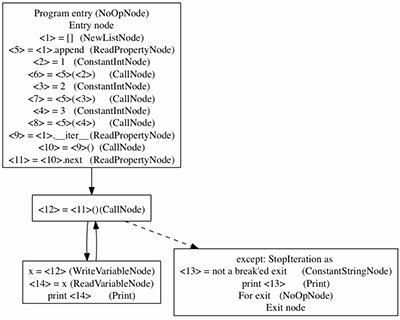
\includegraphics[width=0.48\textwidth]{images/for-example-cfg.png}
	\end{center}
	\vspace{-10pt}
	\caption{Control Flow Graph for the for-loop example \ref{code:forExample}}
	\label{fig:forCfg}
	\vspace{-10pt}
\end{wrapfigure}

First, \inlinecode{expression\_list} is evaluated. This should yield an iterable object, such that an iterator object can be created. Now for each element of the iterator the body of the for loop is evaluated once. As mentioned, if an else block is provided to the loop, it is evaluated when all iterations are done, and the iteration did not stop because of a break statement. \\
To simulate the evaluation sequence of such a for loop in our control flow graph, we need to take a look at the iterator object: to get the next element from a Python iterator object the next method is used. This method returns the next element until the iteration is done and finally raises a \inlinecode{StopIteration} exception. The CFG for the for-loop example \ref{code:forExample} can been seen in figure \ref{fig:forCfg}.

\begin{wrapfigure}{r}{0.5\textwidth}
	\vspace{-20pt}
	\begin{center}
		\includegraphics[width=0.48\textwidth]{images/while.png}
	\end{center}
	\vspace{-10pt}
	\caption{Control Flow Graph for a while-loop}
	\label{fig:whileCfg}
	\vspace{-10pt}
\end{wrapfigure}
For a while loop we generate the control flow graph in figure \ref{fig:whileCfg}.

\section{CFG cunstruction of With statements}
With statements in Python are unlike With statements in JavaScript.\ They are usually used when you have object you need to "open" before you do some work and then "close" it in the end, this pattern is used alot when working with I/O such as files or databases.\ An example of with statements can be seen in Listing \ref{code:withExample}.

\begin{listing}[H]
	\begin{minted}[linenos]{python}
with open('file.txt') as fh:
	print fh.read()
	\end{minted}
	\caption{With example reading a file}\label{code:withExample}
\end{listing}

The formal description of the With statement can be found in The Python Language Reference compound statement list\cite{pyref.compound} section 7.5, the hightlights is that if there is an \inlinecode{as} part of your with statement the result of the method call to \inlinecode{\_\_enter\_\_} assigned to the variable in the with statement. If there is raised an exception during the execution of the body of the With statement it is passed as arguments to the method call \inlinecode{\_\_exit\_\_}, if the result of that call returns something which truth value is \inlinecode{True} the with statement just evaluates normally, If a truth value of \inlinecode{False} is returned the exception isn't caught. If no exceptions happens during execution the \inlinecode{\_\_exit\_\_} method is called, after the body of the With statement, where \inlinecode{None} is passed as arguments.

\section{CFG construction of function and method calls}
\textit{CFG$_{\textit{cond}}$} is the control flow graph that results from the condition. If the condition is the boolean \inlinecode{True}, \textit{CFG$_{\textit{cond}}$} will be the control flow graph consisting of a single node, namely \textit{ConstantBooleanNode}. Inspired from TAJS, Type Analyzer for JavaScript, our \textit{ConstantBooleanNode} holds a result register (\textit{reg$_{\textit{cond}}$} in figure \ref{fig:callCfg}) together with the actual constant value, \inlinecode{True} in this case. \\
The other nodes \textit{ConstantIntNode}, \textit{ConstantFloatNode}, \textit{ConstantLongNode}, \textit{ConstantComplexNode}, \textit{ConstantStringNode}, \textit{ConstantNoneNode}, \textit{NewListNode}, \textit{NewDictionaryNode} and \textit{NewTupleNode} work in a similar way to \textit{ConstantBooleanNode}. \\
The motivation for introducing registers is that a single expression as e.g. \inlinecode{s1.addGrade('math', 10)} is evaluated in several steps. \\
First the function \inlinecode{addGrade} is looked up in the class of \inlinecode{s1}. This is done in the control flow graph using \textit{ReadPropertyNode}, which holds a result register, a base register, i.e. the register where to find the object, and the name of the property to look up. Similar nodes include \textit{ReadVariableNode} and \textit{ReadIndexableNode}. \\
\begin{wrapfigure}{r}{0.5\textwidth}
	\vspace{-20pt}
	\begin{center}
		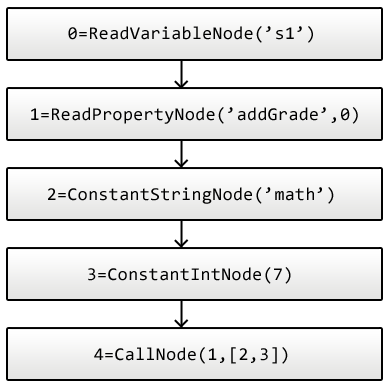
\includegraphics[width=0.48\textwidth]{images/Call-example.png}
	\end{center}
	\vspace{-10pt}
	\caption{Control Flow Graph for a call example}
	\label{fig:callCfg}
	\vspace{-10pt}
\end{wrapfigure}
Secondly, each argument given to the function is evaluated, and finally the actual call is done. Calls in the control flow graph is modeled using the \textit{CallNode}, which holds a result register, a function register and a list of arguments registers. \\
Thus the expression \inlinecode{s1.addGrade('math', 10)} will result in the control flow graph found in figure \ref{fig:callCfg} (where the numbers to the left represent the result registers of the nodes).\\
\todo{Tilfoeje afsnit om \_\_getattribute\_\_ og \_\_getattr\_\_, samt hvordan disse haandteres.} \\
So far we have primarily been concerned with putting constants into registers and reading e.g. variables. In order to support writing we have three different nodes: \textit{WriteVariableNode}, \textit{WritePropertyNode}, and \textit{WriteIndexableNode}. Besides holding a value register, i.e. the register where to find the value being written, \textit{WriteVariableNode} contains the name of the variable being written to, \textit{WritePropertyNode} contains a base register and the property being written to, and \textit{WriteIndexableNode} contains a base and property register (the latter has a register for the property because it is not constant, for instance we could write something like the following: \inlinecode{dict[getKey()] = aValue}, whereas property in \inlinecode{obj.property = aValue} must be a string).

\section{Handling exceptions}
In order to handle the flow caused by exceptions we use two different kinds of edges in the control flow graph. A solid edge indicates normal flow, and a dashed edge indicates exception flow. \\
In Python exceptions can be caught using a try-except-else-finally block. An except block can be annotated with a number of types, and each try-except-else-finally block may contain an arbitrary number of except blocks. As usual, the else block is entered in case of a normal exit, i.e. when no exceptions were raised inside the try block. \\
The AST provided by the Jython parser has been normalized from a try-except-else-finally block into a try-finally block, which contains a try-except-else block in its try block. \\
For instance the code in the first example \ref{code:tryExceptBefore} below is transformed into the code in the next example \ref{code:tryExceptAfter}:

\begin{listing}[H]
	\begin{minted}[linenos]{python}
try:
  <try-stms>
except Foo:
  <except-foo-stms>
except:
  <except-stms>
else: 
  <else>
finally:
  <finally>
	\end{minted}
	\caption{A try-except-else-finally example before convertion}\label{code:tryExceptBefore}
\end{listing}

\begin{listing}[H]
	\begin{minted}[linenos]{python}
try: 
  try:
    <try-stms>
  except Foo:
    <except-foo-stms>
  except:
    <except-stms>
  else:
    <else-stms>
finally:
  <finally-stms>
	\end{minted}
	\caption{A try-except-else-finally example after convertion}\label{code:tryExceptAfter}
\end{listing}

Inductively, CFG's for the statement lists <\inlinecode{try-stms}> (\textit{CFG$_{\textit{try}}$}), <\inlinecode{except-foo-stms}> (\textit{CFG$_{\textit{except-foo}}$}), <\inlinecode{except-stms}> (\textit{CFG$_{\textit{except}}$}), <\inlinecode{else-stms}> (\textit{CFG$_{\textit{else}}$}), and <\inlinecode{finally-stms}> are created. \\
The CFG for the finally block is then cloned into three duplicates (\textit{CFG$_{\textit{finally-normal}}$}, \textit{CFG$_{\textit{finally-handled-exc}}$}, \textit{CFG$_{\textit{finally-unhandled-exc}}$}). The purpose is to have one finally block for each of the following cases: 

\begin{enumerate}
  \item when no exceptions occur during the try block,
  \item when an exception is raised and caught by one of the surrounding except blocks, and no exception is raised from inside that except block, and
  \item when an exception is raised but not caught, which is the case when a) an exception is raised from
the try block and no except blocks handles this particular exception, b) an except block catches an exception raised by the try block, but then raises a new exception on its own.
\end{enumerate}

In particular, it is important that the finally block for handling case (3), i.e. \textit{CFG$_{\textit{finally-unhandled-exc}}$}, is not connected to the exit node of the try-except-else-finally block. Instead, it should be connected to its nearest surrounding except block (if any), or no except block at all (indicating that the program crashes with a runtime error because of an unhandled exception). \\
In the following sections we present the way we generate the CFG of a try-except-else-finally block.

\subsection{The try block}
Each node in \textit{CFG$_{\textit{try}}$} (that does not already have an outgoing exception edge) is connected using an exception edge to the entry node of the first except block (*), in this case the entry node of \textit{CFG$_{\textit{except-foo}}$}. We do not add exception edges to nodes that already have an exception edges, because this would be a loss of information: the control flow always goes to the nearest enclosing except block in case of exceptions. \\
The above models that if an exception occurs during evaluation of one of the statements in a try block, then the control flow will proceed from the first except block. \\
If there is no except blocks, each node should instead be connected using an exception edge to the entry node of its nearest surrounding except or finally block (specifially \textit{CFG$_{\textit{finally-unhandled-exc}}$}). However, we don't add any exception edges here; these will be added inductively because of (*) in case there are any surrounding except or finally blocks.

\begin{wrapfigure}{r}{0.5\textwidth}
	\vspace{-20pt}
	\begin{center}
		\includegraphics[width=0.48\textwidth]{images/Try-except-else-finally.png}
	\end{center}
	\vspace{-10pt}
	\caption{Control Flow Graph for try try-except example \ref{code:tryExceptAfter}}
	\label{fig:tryExceptCfg}
	\vspace{-10pt}
\end{wrapfigure}
\subsection{The except block}
The entry node of each except block is connected using an exception edge to the entry node of the next except block (except for the last block, of course). Thus we make an exception edge from the entry node of \textit{CFG$_{\textit{except-foo}}$} to the entry node of \textit{CFG$_{\textit{except}}$}. \\
We do this because the first except block might not catch the exception (because of the type restrictions), in which the control flow proceeds at the next except block. \\
Furthermore, each node inside the except block should be connected using an exception edge to the entry node of its nearest surrounding except or finally block (specifically \textit{CFG$_{\textit{finally-unhandled-exc}}$}). As above, this is handled inductively. \\
Finally, if an except block actually catches the exception, and no exceptions occur inside that except block, the control flow proceeds to the surrounding finally block (in this case, \textit{CFG$_{\textit{finally-handled-exc}}$}). 

\subsection{The else block}
If no exceptions occur, the else block should be evaluated. Thus we add a normal flow edge from the exit node of \textit{CFG$_{\textit{try}}$} to the entry node of \textit{CFG$_{\textit{else}}$}.\\
Since exceptions may result from evaluating the statements in the else block, each node in \textit{CFG$_{\textit{else}}$} should also be connected to the entry node of the nearest surrounding except or finally block (again, \textit{CFG$_{\textit{finally-unhandled-exc}}$}). \\
In case the evaluation of the statements in the else block does not raise any exceptions, the control flow proceeds either to the exit node of the whole try-except-else block, or in case there is a surrounding finally block, to the entry node of \textit{CFG$_{\textit{finally-normal}}$}.
\chapter{The Analysis Lattice}
Inspired by TAJS we have a lattice for abstract values, $Value$, from which we build a lattice for abstract objects, $Object$. These two lattices are the main building blocks for the lattice of abstract states, $State$. Our analysis lattice is the lattice which for each program point (i.e. for each CFG node) tells the abstract state of that program point. Furthermore the analysis lattice tells the call graph of the CFG.

\section{Abstract Values}
The concrete lattices follows below.

\begin{eqnarray*}
Value = & Undefined \times None \times NotImplemented \times Ellipsis \\
        & \times Boolean \times Integer \times Float \times Long \\
        & \times Complex \times String \times P(ObjectLabel)
\end{eqnarray*}

The value lattice is used to tell the value of a temporary variable (see the lattice $Stack$), and a property on an object (see the lattice $Object$). The $Undefined$, $NotImplemented$, $Ellipsis$ and $None$ lattices all contains two nodes, top and bottom. $NotImplemented$ is a constant in Python that is used sometimes when a function is not supported. $Ellipsis$ is another constant which represents $\dots$ in Python, this constnat is used when indexing using intervals. In Python when a function does not contain a return statement, the constant \inlinecode{None}\cite{pyref.constants} is returned by default, e.g.:

\begin{listing}[H]
	\begin{minted}[linenos]{python}
def a(): pass
a() is None // true
	\end{minted}
	\caption{Constant None}\label{code:NoneExample}
\end{listing}

\begin{wrapfigure}{r}{0.5\textwidth}
	\vspace{-20pt}
	\begin{center}
		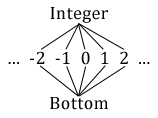
\includegraphics[width=0.48\textwidth]{images/integer-lattice.png}
	\end{center}
	\vspace{-10pt}
	\caption{The integer lattice}
	\label{fig:latticeInteger}
	\vspace{-10pt}
\end{wrapfigure}

Contrary to JavaScript, Python supports integers, floats, longs and complex numbers, so we have separate lattices for those. Note that $Complex = Float \times Float$, since a complex number in Python is represented using a float for the real and imaginary part, respectively \cite{pyref.stdtypes}. The Integer lattice is defined here in figure \ref{fig:latticeInteger}. The $Float$, $Long$ and $String$ lattices are defined in similar ways. Finally, a value can of course also be a pointer to an object on the heap, which we model in the $Value$ lattice by having a power set\footnote{All our power sets are ordered by subset inclusion.} of object labels, $P(ObjectLabel)$.


\section{Abstract State}
We use the following lattice to model abstract state:

\begin{equation*}
State = Heap \times Stack
\end{equation*}

In the following sections the $Heap$ and $Stack$ lattice will be described, but first it is necessary to look at the $Object$ lattice:

\begin{equation*}
Object = (PropertyName \rightarrow Value \times Global) \times P(ObjectLabel^{*})
\end{equation*}

Having made special lattices for the 'primitive' objects there is still a need to handle the more complex objects such as function objects. As with JavaScript you can augment objects with properties at runtime, so the lattice needs to accommodate this dynamic behavior, so we use a map from property names to values. For some objects it is required to track the scope in which they were defined, to model the closure they are evaluated in. Thus the object lattice is the product between object values and a scope chain modelled as a list of object labels.


\section{The Heap}
\begin{equation*}
Heap = (ObjectLabel \rightarrow Object)
\end{equation*}

The heap is modelled by a map from object labels to an object value. We found it benefitial to distinguish between different types of objects but still handle them in the same way in the heap. To achieve this we made several different subclasses to the object label object, e.g. function object, which besides its name also holds a reference to the CFG node that is the entry node for that function.


\section{The Stack}
The $Stack$ lattice is defined as:

\begin{equation*}
Stack = (TempVar \rightarrow Value) \times P(ObjectLabel^{*})
\end{equation*}

For each temporary variable we specify the value of that particular temporary variable. The power set $P(ObjectLabel^{*})$ specifies the scope chain ($ObjectLabel^{*}$). The head element in the scope chain determines which object on the heap, local variable writes should we written to. For instance we will for each program have an object on the heap, that models the module/top-level script environment \inlinecode{\_\_main\_\_}\cite{pyref.main} (this is what corresponds to the global object in JavaScript). Whenever an assignment to a variable occurs in the top-level scripting environment, e.g. \inlinecode{x=10}, the variable \inlinecode{x} is set as a property mapping to the integer 10 on the \inlinecode{\_\_main\_\_} object in the heap.

The scope chain specifies where to look in case of e.g. reading a variable that is not present on the variable object. The following simple example can be used to illustrate this:

\begin{listing}[H]
	\begin{minted}[linenos]{python}
x = 10
def a():
	return x
a() # 10
	\end{minted}
\caption{Scope example}\label{code:ScopeExample}
\end{listing}

For this particular scope example we will have the following objects on the heap:

\begin{enumerate}
  \item The \inlinecode{\_\_main\_\_} object,
  \item The object of the function \inlinecode{a},
  \item The function wrapper object of \inlinecode{a}, and
  \item The scope object of \inlinecode{a} (which is an object similar to the \inlinecode{\_\_main\_\_} object, i.e. an object where local variables are written onto).
\end{enumerate}

When entering the function (calling it) the scope object of the function a (or more precise, its label) will be pushed onto the current scope chain (which at the function call will be the list containing the \inlinecode{\_\_main\_\_} object). When the variable \inlinecode{x} is read, \inlinecode{x} is looked up in the scope chain starting from the head of it. For this particular example \inlinecode{x} is found on the \inlinecode{\_\_main\_\_} object. In the next chapter we describe our work towards handling functions including why we need these three different kinds of objects on the heap. Handling functions of course includes populating the call graph such that the CFG becomes interprocedural.

\begin{eqnarray*}
CallGraph = & (Node \times Node) \\
Analysis = & (Node \rightarrow State) \times CallGraph
\end{eqnarray*}

\chapter{Results}
\label{chapter:results}
In this report we have presented one approach to a type analyser for Python, capable of analysing simple Python programs. In this chapter we will give examples of some small non-trivial programs together with the results from our type analyser. The primary goal was to support simple usage of the magic method \inlinecode{\_\_getattr\_\_} similar to the way it was used in Django \cite{django}.

%During our project we have developed a type analyser for Python, which is able to analyse simple Python programs. In this section we present some small, but non-trivial to %analyse, programs together with the results of our type analyser. We aimed to be able to support simple use of the magic method \inlinecode{\_\_getattr\_\_}, as we found that %all uses of it in the web framework Django\cite{django} were simple.

In order to achieve this goal limited support for exceptions was needed. Consider the following calculator example that makes use of exceptions for unsupported operations:

\begin{listing}[H]
	\begin{minted}[linenos]{python}
def calculator(a, op, b):
  if (op == "+"): result = a + b
  elif (op == "-"): result = a - b
  elif (op == "*"): result = a * b
  elif (op == "/"): result = a / b
  else: raise Exception()
  return result

try:
  amodb  = calculator(10, "%", 20)
except:
  err = "An error occured"
	\end{minted}
\end{listing}

For this example our analyser will conclude that \inlinecode{amodb} is undefined and that \inlinecode{err} is "An error occurred". Due to a very simple path sensitivity our analyser doesn't conclude that \inlinecode{amodb} is either undefined, \inlinecode{a}+\inlinecode{b}, \inlinecode{a}-\inlinecode{b}, \inlinecode{a}*\inlinecode{b} or \inlinecode{a}/\inlinecode{b}. By changing line 15 to \inlinecode{calculator(10, "+", 20)} our analyser would conclude that the result of the function call would be 30.

The limited exception handling has enabled us to support implicit \inlinecode{\_\_getattr\_\_} calls. Consider part of the \inlinecode{Student} example from \autoref{Features} about dynamic features that uses the magic method \inlinecode{\_\_getattr\_\_}:

\begin{listing}[H]
	\begin{minted}[linenos]{python}
class Student(object):
  def __init__(self, name):
    self.name = name
  def __getattr__(self, name):
    if name in self.grades:
      return self.grades[name]
    else:
      raise AttributeError()
a = Student('John')
a.grades = { 'math': 'A' }
try:
  mathgrade = a.math
except:
  err = "Error"
	\end{minted}
\end{listing}

Our tool is able to analyse this program and conclude that \inlinecode{mathgrade} is either \inlinecode{'A'} or \inlinecode{undefined} (the latter because we do a weak update in line 10 to \inlinecode{a.grades}). It should be mentioned, that the lack of context sensivity destroys the precision very quickly because Python has a lot of implicit method calls, contrary to JavaScript.

Dynamically expanding the \textit{ReadAttributeNode} results in 12 added CFG nodes per expanded \textit{ReadAttributeNode}, however it can be avoid when it can be statically determined that the attribute is definitely present. It would be nice to give a measure of how often the dynamic expansion can be avoided, but because our current analyser doesn't make any strong updates on classes it always does the expansion, except when we make use of the assumption mentioned in \autoref{Magic methods transformation}.

It is important to stress the fact that we only support a subset of Python. Not supporting the magic method \inlinecode{\_\_getattribute\_\_} simplifies the situation as discussed in \autoref{Magic methods transformation}.
\chapter{Further work}

\todo{andre magic methods}

\begin{thebibliography}{8}

\bibitem{tajs} Simon Holm Jensen, Anders M\o ller and Peter Thiemann. Type Analysis for JavaScript. \url{http://www.brics.dk/TAJS/}.
\bibitem{sa} Anders M\o ller and Michael I. Schwartzbach. Static Program Analysis. Department of Computer Science, Aarhus University, Denmark. January 30, 2013.
\bibitem{lamdapy} Shriram Krishnamurthi and Joe Gibbs Politz et. al. Python: The Full Monty, submitted OOPSLA 2013 paper, March 28, 2013
\bibitem{jython} The Jyhton Project: Python for the Java Platform \url{http://www.jython.org/}, June 26, 2013
\bibitem{pyref.datamodel} The Python Language Reference, Datamodel \url{http://docs.python.org/2/reference/datamodel.html}, May 13, 2013
\bibitem{pyref.constants} The Python Language Reference, Constants \url{http://docs.python.org/2/library/constants.html}, May 13, 2013
\bibitem{pyref.stdtypes} The Python Language Reference, Built-in Types \url{http://docs.python.org/2/library/stdtypes.html}, May 13, 2013
\bibitem{pyref.main} The Python Language Reference, \_\_main\_\_ \url{http://docs.python.org/2/library/__main__.html}, May 13, 2013
\bibitem{pyref.compound} The Python Language Reference, Compound Statements \url{http://docs.python.org/2/reference/compound_stmts.html}, May 20, 2013
\bibitem{pyref.typehierarchy} The Python Language Reference, The standard type hierarchy \url{http://docs.python.org/2/reference/datamodel.html#the-standard-type-hierarchy}, June 9, 2013
\bibitem{pyref.c3mro} The C3 method resolution order \url{http://www.python.org/download/releases/2.3/mro/}, June 9, 2013
\bibitem{recency} Gogul Balakrishnan and Thomas Reps. Recency-Abstraction for Heap-Allocated Storage \url{http://link.springer.com/chapter/10.1007/11823230_15}, June 10, 2013
\bibitem{lambdapy} Python: The Full Monty \url{http://cs.brown.edu/research/plt/dl/lambda-py/ae/index.html}, June 10, 2013
\bibitem{tool.pep8} pep8 - Python style guide checker \url{https://pypi.python.org/pypi/pep8}, June 26, 2013
\bibitem{tool.pyflakes} pyflakes - passive checker of Python programs \url{https://pypi.python.org/pypi/pyflakes}, June 26, 2013
\bibitem{tool.pychecker} PyChecker - Python source code checking tool \url{https://pypi.python.org/pypi/PyChecker}, June 26, 2013
\bibitem{tool.pylint} Pylint - python code static checker \url{https://pypi.python.org/pypi/pylint}, June 26, 2013
\bibitem{ide.appcelerator} Appcelerator: PyDev \url{http://pydev.org/}, June 26, 2013
\bibitem{ide.jetbrains} JetBrains. PyCharm \url{http://www.jetbrains.com/pycharm/}, June 26, 2013
\bibitem{ide.wingware} Wingware \url{http://wingware.com/}, June 26, 2013
\bibitem{django} Django \url{https://www.djangoproject.com/}, June 26, 2013
\bibitem{aopas} D.R. Chase, M. Wegman, and F. Zadeck. Analysis of pointers and structures. In \textit{Prog. Lang. Design and Impl.} pages 296-310, 1990.
\bibitem{starkiller} Michael Salib. Faster than C: Static type inference with Starkiller. \url{http://citeseer.ist.psu.edu/viewdoc/summary?doi=10.1.1.95.3786}, June 27, 2013
\end{thebibliography}


\backmatter

\appendix

\chapter{Complete node reference}
\label{chapter:NodeRef}

\begin{description}
	\item[FunctionDeclNode \inlinecode{def f(...):}] Used when a function is defined, the node holds references to the function entry node and the exit node. The registers of all the default arguments is also kept in this node.
	\item[ClassDeclNode \inlinecode{class c(...):}]  
	\item[ClassEntryNode]
	\item[FunctionEntryNode] 
	\item[ExitNode] 
	\item[ConstantBooleanNode] Used when boolean values are created. Since \inlinecode{False} and \inlinecode{True} is not keywords in Python but just variables. The node is only used when CFG rewrites. \todo{This is related to issue \#1 once this is removed the ConstantBooleanNode can be removed}
	\item[ConstantIntNode] Introduces integers from the AST into the CFG.
	\item[ConstantFloatNode] Introduces floats from the AST into the CFG.
	\item[ConstantLongNode] Introduces longs from the AST into the CFG.
	\item[ConstantComplexNode] Introduces complex numbers from the AST into the CFG.
	\item[ConstantStringNode] Introduces strings from the AST into the CFG.
	\item[ConstantNoneNode] \inlinecode{None} is not a keyword in Python but just variables, so the Node is only introduced when certain CFG constructions is created. An example would be when declaring a function here a hardcoded return node is put in the end with the value of a \textit{ConstantNoneNode}.
	\item[ReadVariableNode \inlinecode{x}] Introduced when reading variables.
	\item[ReadPropertyNode \inlinecode{reg$_{\inlinecode{obj}}$.property}] Introduced when reading a property on an object.
	\item[ReadIndexableNode \inlinecode{reg$_{\inlinecode{obj}}$[reg$_{\inlinecode{index}}$]}] Introduced when reading a indexable attribute on an object.
	\item[WriteVariableNode \inlinecode{x = value}] Introduced when writing to variables
	\item[WritePropertyNode \inlinecode{reg$_{\inlinecode{obj}}$.property = value}] Introduced when writing to a property on an object.
	\item[WriteIndexableNode \inlinecode{reg$_{\inlinecode{obj}}$[reg$_{\inlinecode{index}}$]}] Introduced when writing a indexable attribute on an object.
	\item[DelVariableNode \inlinecode{del x}] Introduced when deleting a variable from the current scope.
	\item[DelVariableNode \inlinecode{del reg$_{\inlinecode{obj}}$.property}] Introduced when deleting a property on an object.
	\item[DelIndexableNode \inlinecode{reg$_{\inlinecode{obj}}$[reg$_{\inlinecode{index}}$]}] Introduced when deleting a indexable attribute on an object.
	\item[NoOpNode \inlinecode{pass}] Introduced when \inlinecode{pass} is parsed in the AST. The \textit{NoOpNode} is also used when constructing the CFG as fill. Since the \textit{NoOpNode} dosen't do anything in the further analysis a minifier is created to remove these nodes from the CFG.
	\item[CallNode \inlinecode{reg$_{\inlinecode{function}}$(reg$_{\inlinecode{1}}$, ..., reg$_{\inlinecode{n}}$)}] Used when a function call happens. The node contains the function register and the lists of all the arguments.
	\item[AfterCallNode] Introduced after each CallNode and holds the register of the result.
	\item[ReturnNode \inlinecode{return reg$_{\inlinecode{value}}$}] Introduced whenever there is a \inlinecode{return} statement in the AST. 
	\item[CompareOpNode \inlinecode{reg$_\inlinecode{left}$ op$_\inlinecode{comp}$ reg$_\inlinecode{right}$}] Introduced when there is made compare expressions is created in the AST.
	\item[BinOpNode \inlinecode{reg$_\inlinecode{left}$ op$_\inlinecode{binop}$ reg$_\inlinecode{right}$}] Introduced when there is made binary operation expressions is created in the AST.
	\item[IfNode \inlinecode{if reg$_\inlinecode{cond}$:}] Introduced when making \inlinecode{if} statements in the code. IfNodes is also introduced in other CFG constructions such as \inlinecode{while} statements and \inlinecode{binary} expressions.
	\item[RaiseNode \inlinecode{raise reg$_\inlinecode{exception}$}] Introduced when exceptions is thrown in the AST. The node can hold the register containing the exception. If the register isn't set its a re-raise exception.
	\item[ExceptNode \inlinecode{except (type$_\inlinecode{1}$, ..., type$_\inlinecode{n}$)}:] Introduced when exceptions is cought after a \inlinecode{try} statement in the AST.
\end{description}



\end{document}
